En la siguiente sección se podrá observar una breve descripción del modelo de datos a usar. Los autores han decidido usar una base de datos orientada a grafos, Neo4j, por lo cual cada explicación se hará a grandes rasgos sobre un grafo ejemplo generado directamente en Neo4j.

Otro dato a tener en cuenta será que los autores \textbf{sólo describirán el modelo de datos que se ajusta, según ellos, a las funcionalidades a ser implementadas}.

En el capítulo \ref{chap:anexos} el lector podrá encontrar en detalle la descripción de cada nodo etiqueta.

\section{Modelo de datos de gestión de eventos}


\begin{figure}[!htb]
  \begin{center}
    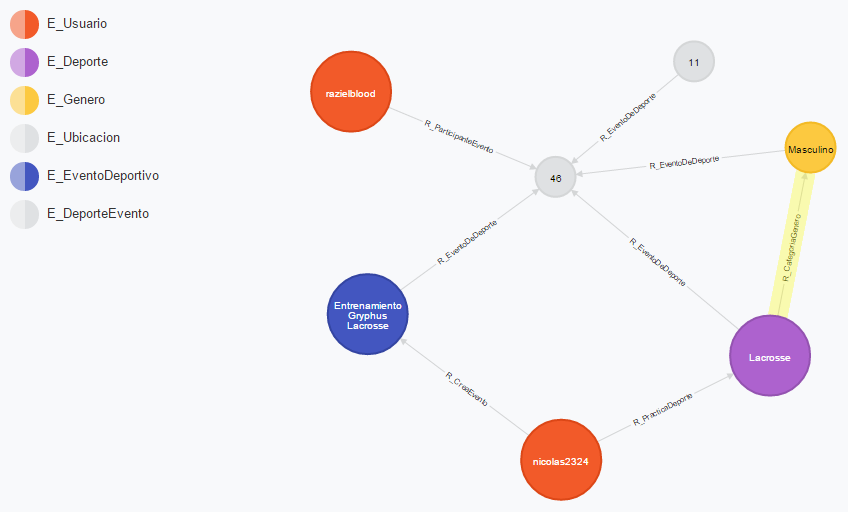
\includegraphics[width=11cm]{./imagenes/Modelo_de_datos/Gestion_eventos.png}
    \caption{Modelo de datos de gestión de eventos}
    \label{fig:modelo_datos_gestion_eventos}
    \textbf{Fuente:}  Autores
  \end{center}
\end{figure}

\section{Modelo de datos de gestión de ubicaciones}


\begin{figure}[!htb]
  \begin{center}
    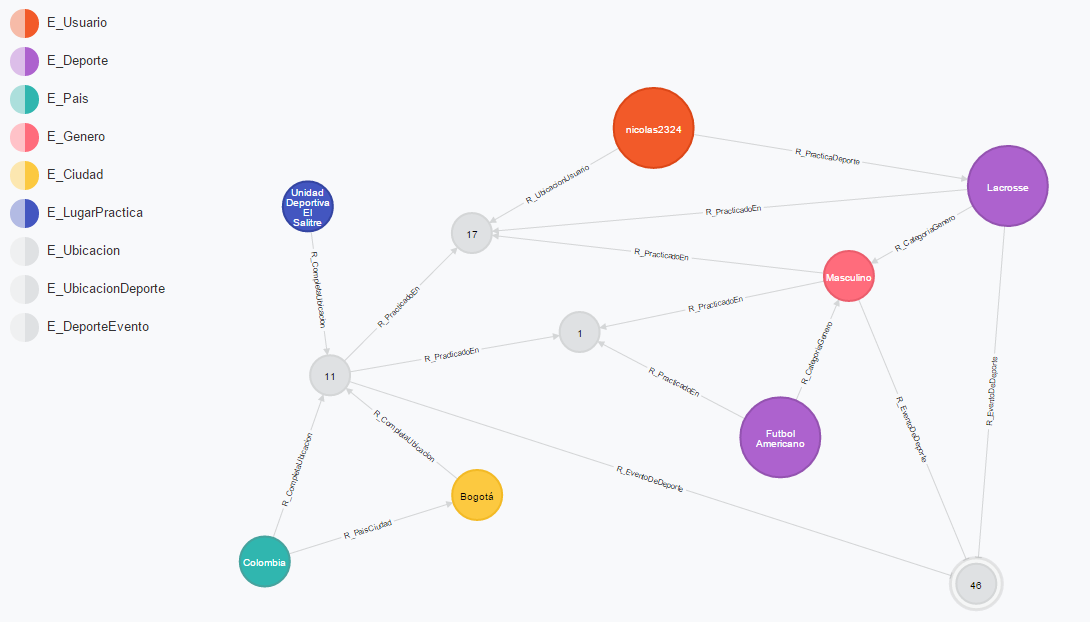
\includegraphics[width=11cm]{./imagenes/Modelo_de_datos/Gestion_ubicaciones.png}
    \caption{Modelo de datos de gestión de ubicaciones}
    \label{fig:modelo_datos_gestion_ubicaciones}
    \textbf{Fuente:}  Autores
  \end{center}
\end{figure}

\section{Modelo de datos de gestión de deportes}


\begin{figure}[!htb]
  \begin{center}
    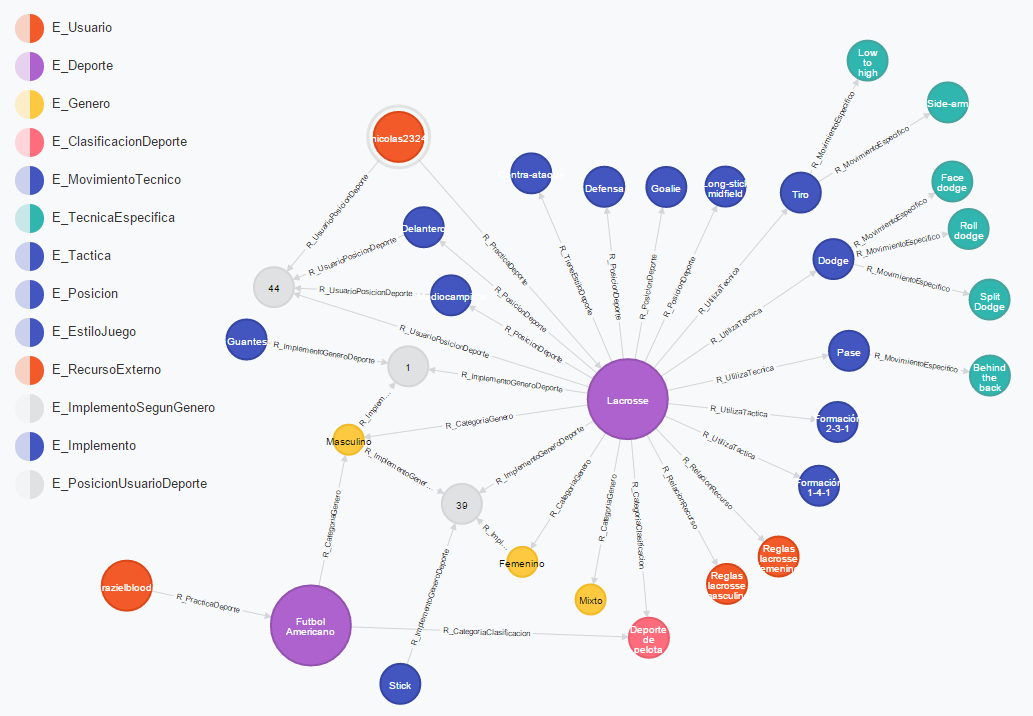
\includegraphics[width=11cm]{./imagenes/Modelo_de_datos/Gestion_deportes.png}
    \caption{Modelo de datos de gestión de deportes}
    \label{fig:modelo_datos_gestion_deportes}
    \textbf{Fuente:}  Autores
  \end{center}
\end{figure}